\PassOptionsToPackage{pdftex}{graphicx} % pdftex hack fuer graphicx
\documentclass[pdftex,hyperref=pdftex,12pt,aspectratio=169]{beamer}
\mode<presentation>
{
\usetheme{Warsaw}
\setbeamercovered{invisible}
}
%\usetheme[fakultaet-oder-cau]{CAU2013}
\usepackage[style=authoryear,citestyle=authoryear,backend=biber]{biblatex}
\addbibresource{references.bib}

\renewcommand{\bibfont}{\ttfamily}

\usepackage{listings}

\usepackage[utf8]{inputenc}
\usepackage[T1]{fontenc}
\usepackage[american]{babel}
\usepackage{csquotes}
\usepackage{mathabx}

\usepackage[scaled=0.8]{beramono}

\usepackage{todonotes}
\usepackage{multicol}
\usepackage{xcolor}
\newcommand\mynote[1]{\textcolor{red}{#1}}
\newcommand{\semitransp}[2][35]{\textcolor{fg!#1}{#2}}
%\usepackage[notocbib]{apacite}

% Variable width block
\newenvironment<>{varblock}[2][0.9\textwidth]{%
    \setlength{\textwidth}{#1}%
    \setlength{\linewidth}{\textwidth}% required to itemize respect the width of block
  \begin{actionenv}#3%
    \def\insertblocktitle{#2}%
    \par%
    \usebeamertemplate{block begin}}
  {\par%
  \usebeamertemplate{block end}%
  \end{actionenv}}

% Variable width example block
\newenvironment<>{varexampleblock}[2][0.9\textwidth]{%
    \setlength{\textwidth}{#1}%
    \setlength{\linewidth}{\textwidth}%
  \begin{actionenv}#3%
    \def\insertblocktitle{#2}%
    \par%
    \setbeamercolor{local structure}{parent=example text}%
    \usebeamertemplate{block example begin}}
  {\par%
  \usebeamertemplate{block example end}%
    \end{actionenv}}

% Variable width alert block
\newenvironment<>{varalertblock}[2][0.9\textwidth]{%
    \setlength{\textwidth}{#1}%
    \setlength{\linewidth}{\textwidth}%
  \begin{actionenv}#3%
    \def\insertblocktitle{#2}%
    \par%
    \setbeamercolor{local structure}{parent=alerted text}%
    \usebeamertemplate{block alerted begin}}
  {\par%
  \usebeamertemplate{block alerted end}%
    \end{actionenv}}

%% Beamer Bibliography Fix
%\def\newblock{\hskip .11em plus .33em minus .07em}
%\bibliographystyle{alpha}

\makeatletter

\makeatother

%% title setup

\title{Course-Software-Testing}
\subtitle{MarDATA} 
\author[Prigge, Rath, Hiremath, Gundlach]{Enno Prigge \and Willi Rath \and Dilip Hiremath \and Sven Gundlach\\[3mm]Kiel University}
\date[18-11-2020]{18\textsuperscript{th} November 2020}

\AtBeginSection[]
{
\begin{frame}<beamer>
\frametitle{Structure}
\tableofcontents[currentsection, subsectionstyle=hide]
\end{frame}
}

%% language settings
\selectlanguage{american}

\begin{document}

%% remove Figure from caption
\setbeamertemplate{caption}{\raggedright\insertcaption\par}
\setbeamertemplate{navigation symbols}{}%remove navigation symbols



%\ttfamily

% -----------------------------------------

%% make titleslide
{
\begin{frame}[plain]{}{}%
\titlepage
\begin{pgfpicture}{0cm}{0cm}{\textwidth}{1cm}
\pgfline{\pgfxy(0,0)}{\pgfxy(15.5,0)}
\pgfputat{\pgfxy(0,-0.2)}{\pgfbox[left,top]{\pgfimage[width=25mm]{images/MarDATA_logo}}}
\pgfputat{\pgfxy(5.8,-0.1)}{\pgfbox[left,top]{
% \begin{minipage}{95mm}
% \tiny footer
% \end{minipage}
}}
\end{pgfpicture}
\end{frame}
}

\begin{frame}
\frametitle{Structure}
\tableofcontents[subsectionstyle=hide]
 % You might wish to add the option [pausesections]
\end{frame}

%%%%%%%%%%%%%%%%%%%%%%%%%%%%%%%%%

\section{Introduction}
\subsection{What is software testing?}

%%%%%%%%%%%%%%%%%%%%%%%%%%%%%%%%%

\begin{frame}[fragile]
\frametitle{What is software testing?}

\begin{block}{Testing:}
\begin{itemize}
\item Testing is the process of executing a program with the intent of finding errors \semitransp{(Myers, G.J., 1979. The Art of Software Testing John Wiley and Sons Ltd.)}
\item Software testing is the process of exercising or evaluating a system or system component by manual or automated means to verify that it satisfies specified requirements. \semitransp{(IEEE 83a)}
\end{itemize}
\end{block}

\pause

\begin{block}{Principle of Testing:}
Testing can show presence of bugs but not absence or a proof of correctness. No bug found shows not a correct system.
\end{block}

\end{frame}

%%%%%%%%%%%%%%%%%%%%%%%%%%%%%%%%%

\begin{frame}
\frametitle{New features: \glqq Naive\grqq\ Workflow}
 
Typical  \glqq unstructured \grqq\ approach:
\begin{itemize}
   \item Implementation of new features
   \item Call and test of features from main method, output with \textbf{System.out.println}
   \item Manual check whether results are correct (or at least plausible)
   \item Test code in Main method is not used later
\end{itemize}
 
 \pause
 
Cons?
 \begin{itemize}
	 \item Code in Main method not  \glqq belonging there\grqq
		\item Test code is discarded, although it is still useful later
		\item Tests are no longer executed
   \item[$\rightarrow$] Regressions are not recognized
\end{itemize}
\end{frame}

%%%%%%%%%%%%%%%%%%%%%%%%%%%%%%%%%

\subsection{Techniques $\&$ Approaches}

%%%%%%%%%%%%%%%%%%%%%%%%%%%%%%%%%

\begin{frame}
\frametitle{Testing Techniques}
  \begin{center}
  \pgfimage[width=.55\textwidth]{images/Einleitung/abbildungen/test_technique}
  \end{center}
\end{frame}

%%%%%%%%%%%%%%%%%%%%%%%%%%%%%%%%%

\subsection{Testing Approaches}

%%%%%%%%%%%%%%%%%%%%%%%%%%%%%%%%%

\begin{frame}[fragile]
\frametitle{Testing Approaches}

\begin{itemize}
\item<1-> Level of \alert<1>{knowledge} and \alert<1>{access} to implementation
\begin{itemize}
\item Whitebox Testing
\item Blackbox Testing
\end{itemize}
\end{itemize}

\begin{minipage}[t]{0.49\textwidth}
\begin{itemize}
\item<2-> \alert<2>{Testing scope}
\begin{itemize}
\item System testing
\item Module testing
\item Integration testing
\item Unit testing
\end{itemize}
\end{itemize}
\end{minipage}
%
\begin{minipage}[t]{0.49\textwidth}
\begin{itemize}
\item<3-> \alert<3>{Concepts}
\begin{itemize}
\item Regression Testing
\item Fuzzing
\item Metamorphic testing
\item Design by Contract
\item Machine Learning
\item \ldots
\end{itemize}
\end{itemize}
\end{minipage}

\end{frame}

%%%%%%%%%%%%%%%%%%%%%%%%%%%%%%%%%

\subsection{Test Oracle}

%%%%%%%%%%%%%%%%%%%%%%%%%%%%%%%%%

\begin{frame}
\frametitle{Test Oracle}
  \begin{center}
  \pgfimage[width=0.6\textwidth]{images/Qualitaetssicherung/abbildungen/TestOracle}
  \end{center}
\end{frame}

%%%%%%%%%%%%%%%%%%%%%%%%%%%%%%%%%

\begin{frame}
\frametitle{Concepts by type of Test Oracle}
  \begin{center}
  \pgfimage[width=0.55\textwidth]{images/Einleitung/abbildungen/tr3}
  \end{center}
\end{frame}
%%%%%%%%%%%%%%%%%%%%%%%%%%%%%%%%%

\subsection{Test driven development}

%%%%%%%%%%%%%%%%%%%%%%%%%%%%%%%%%

\begin{frame}[fragile]

\begin{block}{Test driven Development:}
Software development approach in which a test is written before writing the code
\end{block}

\end{frame}

%%%%%%%%%%%%%%%%%%%%%%%%%%%%%%%%%

\begin{frame}[fragile]
\begin{block}{Definitions of terms}
\begin{enumerate}[align=parleft]
\item [\small Test Condition:] What needs to be tested. \alert<1>{Item} or event that could be \alert<1>{verified}.
\item [\small Test case:] \alert<2>{Testing test condition} or objectives, consist of input values, preconditions, expected results, post conditions.
\item [\small Test procedure:] \alert<3>{Collection} of test cases arranged in sensible order to execute a test.
\item [\small Test suite:] \alert<4>{Entire} test.
\item [\small Test data:] \alert<5>{Input} data for a test case.
\item [\small Expected result:] \alert<6>{Outputs}, changes to data and states and other consequences anticipated to happen.
\item [\small Test script:] \alert<7>{Automated} test procedure.
\end{enumerate}
\end{block}
\end{frame}
%%%%%%%%%%%%%%%%%%%%%%%%%%%%%%%%%

\begin{frame}
\frametitle{Test driven development process}
  \begin{center}
  \pgfimage[width=1.\textwidth]{images/Einleitung/abbildungen/test_development_process}
  \end{center}
\end{frame}
%%%%%%%%%%%%%%%%%%%%%%%%%%%%%%%%%%

\subsection{Testing Activities}

%%%%%%%%%%%%%%%%%%%%%%%%%%%%%%%%%

\begin{frame}[fragile]

\begin{block}{Activities involved in testing}
\begin{enumerate}[align=parleft]
\item [\small Test Planning:] Evaluate the risk of the software and understand the objectives that define test specifications.
\item [\small Test Design:] Identification of test conditions based on specifications, behavior and structure of the software.
\item [\small Test Impl.:] Test implementation: implement test cases, prioritize and organize test procedure, prepare execution
\item [\small Test Eval.:] Execute test, record the identities and versions of the software under test. Compare actual results of what happen with expected results.
\item [\small Test Closure:] End of a testing phase or entire project testing. Check deliverable have been accepted and signed of. Archive the test.
\end{enumerate}
\end{block}
\end{frame}
%%%%%%%%%%%%%%%%%%%%%%%%%%%%%%%%%

\subsection{Test coverage}

%%%%%%%%%%%%%%%%%%%%%%%%%%%%%%%%%

\begin{frame}[fragile]
\frametitle{Risk mitigation}
\begin{block}{How much testing is enough?}
\begin{enumerate}[align=parleft]
\item [\small Exhaustive test:] Test approach in which the test suite comprises all combinations of input values and preconditions.
\begin{itemize}
\item \alert{Not feasible} except for trivial cases
\end{itemize}
\item [\small Risk mitigation:] Use risks and \alert{priorities to focus} testing efforts.
\begin{itemize}
\item Impossible to understand all end user scenarios
\item Impossible to analyze all implications of code changes
\item [\small Automation:] Automated testing can have significant coverage
\end{itemize}
\end{enumerate}
\end{block}

\end{frame}

%%%%%%%%%%%%%%%%%%%%%%%%%%%%%%%%%

\begin{frame}
\frametitle{Equivalence Class Partitioning}
\begin{block}{Aim}
\alert{Divide} input \alert{parameter} and output  ranges into equivalence classes.
%Divide the definition ranges of input parameters and value ranges of output parameters into equivalence classes from which test cases can be derived.
\end{block}
 
\vspace{\baselineskip}
\begin{block}{Assumption}
When processing a representative from an equivalence class, a program \alert{behaves the same way as with all other values} from this equivalence class.
\end{block}
 
\vspace{\baselineskip}
\begin{block}{Representative value for a test case}
Any representative value from each class.
\end{block}
\end{frame}

%%%%%%%%%%%%%%%%%%%%%%%%%%%%%%%%%

\begin{frame}
\frametitle{Boundary Value Analysis}
\begin{itemize}
  \item Test cases that cover the boundary values of equivalence classes or that are in the \alert{immediate vicinity of the boundaries} uncover errors very often.
  \item \alert{Not any element} from the equivalence class is valid as representative for all boundaries.
  \item Pick one or more \alert{elements such that every boundary} of the equivalence class is tested.
\end{itemize}
\end{frame}

%%%%%%%%%%%%%%%%%%%%%%%%%%%%%%%%%

\begin{frame}
\frametitle{Equivalence classes with boundary values}
\begin{center}
\pgfimage[width=0.95\textwidth]{images/Qualitaetssicherung/abbildungen/AequivalenzklassenMitGrenzwerten}
\end{center}
\end{frame}
%\include{eng/05_Technique}
%%%%%%%%%%%%%%%%%%%%%%%%%%%%%%%%%

\section{Whitebox \& Blackbox Testing}

%%%%%%%%%%%%%%%%%%%%%%%%%%%%%%%%%

\begin{frame}
  \begin{center}
  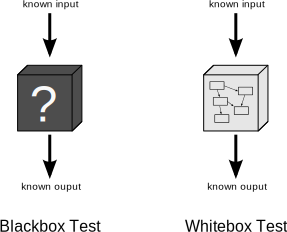
\includegraphics[width=.5\textwidth]{images/Qualitaetssicherung/abbildungen/BlackBoxAndWhiteBoxTesting}
  \end{center}
\end{frame}

%%%%%%%%%%%%%%%%%%%%%%%%%%%%%%%%%

\subsection{Whitebox Testing}

%%%%%%%%%%%%%%%%%%%%%%%%%%%%%%%%%
\begin{frame}
\frametitle{Whitebox Testing of Modules}
\framesubtitle{testing in the small}
\begin{description}[Anwei]
  \item[Statement Coverage:] \hfill \textbf{Statement coverage criterion}
  \begin{itemize}
    \item [] \small All executable statements in the source code are executed at least once.
  \end{itemize}
  \item[Edge coverage:] \hfill \textbf{Edge-coverage criterion}
  \begin{itemize}
    \item [] \small Each edge of the control graph being traversed at least once.
  \end{itemize}
  \item[Path (Branch) Coverage:] \hfill \textbf{Path-coverage criterion}
  \begin{itemize}
    \item [] \small All paths leading from the initial to the final node of the control graph being traversed.
  \end{itemize}
  \item[(Compound) Condition Coverage:] \hfill \textbf{Condition coverage criterion}
  \begin{itemize}
    \item [] \small Each possible combination of conditions must be executed at least once.
  \end{itemize}
\end{description}
\end{frame}

%%%%%%%%%%%%%%%%%%%%%%%%%%%%%%%%%

\subsection{Blackbox Testing}

%%%%%%%%%%%%%%%%%%%%%%%%%%%%%%%%%
\begin{frame}
\frametitle{Blackbox Testing of modules}
\framesubtitle{testing in the large}
\begin{enumerate}[align=parleft]
  \item [Idea:] A part of a program is tested without knowledge of the internal implementation.
  \item [Problem:] How to define the test set? 
  \begin{itemize}
  \item [] Defining the test set can only rely on the specification.
  \item [] Formal specifications are then a prerequisite for the systematic generation of test sets.
  \end{itemize}
\end{enumerate}
\end{frame}

%%%%%%%%%%%%%%%%%%%%%%%%%%%%%%%%%

\begin{frame}
\frametitle{Blackbox Testing of modules (contd.)}

\begin{enumerate}[align=parleft]
  \item [Method:] Derive test cases from the program specification.
  \begin{itemize}
  \item [] Disregard program structure.
  \end{itemize}
  \item [Pro:] Comprehensive but low-redundancy testing of the specified functionality.
  \begin{itemize}
  \item [] The key factor is the functional coverage.
  \end{itemize}
  \item [Con:] Oversight of functionality.
\end{enumerate}
\begin{block}{Defining a test case:}
    \begin{itemize}
      \item Functional equivalence class formation (equivalence class partitioning)
      \item Boundary value analysis (BVA)
      \item Special value testing
    \end{itemize}
\end{block}
\end{frame}
%%%%%%%%%%%%%%%%%%%%%%%%%%%%%%%%%

\section{Mocking}

%%%%%%%%%%%%%%%%%%%%%%%%%%%%%%%%%

\subsection{Categories}

%%%%%%%%%%%%%%%%%%%%%%%%%%%%%%%%%
\begin{frame}
 \frametitle{Mock objects: Categories}
 \footnotesize
 \begin{description}
  \item[Dummy objects] are passed around but never actually used. Usually they are just used to fill parameter lists.
  \item[Fake objects] actually have working implementations, but usually take some shortcut which makes them not suitable for production (an in-memory database is a good example).
  \item[Stubs] provide canned answers to calls made during the test, usually not responding at all to anything outside what's programmed in for the test.
  \item[Spies] are stubs that also record some information based on how they were called.
  \item[Mocks] are [\dots] objects pre-programmed with expectations which form a specification of the calls they are expected to receive.
 \end{description}
\end{frame}

%%%%%%%%%%%%%%%%%%%%%%%%%%%%%%%%%

\subsection{Summary}

%%%%%%%%%%%%%%%%%%%%%%%%%%%%%%%%%

\begin{frame}
 \frametitle{Mocking: Summary}
 
\begin{description}
\item [Motivation:] \alert{Replace} complex objects for test:
\begin{itemize}
  \item Simulation
  \item Replace with dummies
  \item Collect additional debug information
\end{itemize}
\item [Connection to Unit-Testing:] \alert{Extends assertions} by Verification. Testing of interactions with mock objects.
\item [Verification:]
\begin{itemize}
  \item [] Mock objects log function calls. This allows to check properties of the \textit{stack trace (call history)} of mock objects.
  \item [] \alert{No formal verification}
\end{itemize}
\item [Unit Tests \textit{vs.} Mock-Verification?] \alert{Addition, not replacement} but different aspects.
\end{description}
\end{frame}
%%%%%%%%%%%%%%%%%%%%%%%%%%%%%%%%%

\section{Unit Test}

%%%%%%%%%%%%%%%%%%%%%%%%%%%%%%%%%

\begin{frame}
 \frametitle{Unit Test}
  \scriptsize
 \begin{description}
 \item [Automatic unit tests:] \hfill
  \begin{itemize}
  \item Test code in a specially designated area of the project
  \item Execution like \alert{Main methods} but tool support for:
  \begin{itemize}
    \item Comparison with expected behavior
    \item automatic execution of all tests
    \item Statistics on completed and failed tests
   \end{itemize}
\end{itemize}
\end{description}
 \pause
 
 \begin{description}
 \item [Pros:] \hfill
\begin{itemize}
   \item Separation of functionality and tests
   \item Tests are retained
   \item Tests can be run continuously, automatically\\
      $\rightarrow$ Regressions are identified
   \item Tests as \alert{quality gateway} for integration of new code into the master branch or master repository
\end{itemize}
\end{description}
\end{frame}

%%%%%%%%%%%%%%%%%%%%%%%%%%%%%%%%%

\subsection{Demo}

%%%%%%%%%%%%%%%%%%%%%%%%%%%%%%%%%

\begin{frame}[containsverbatim]{An Demo-function}
\scriptsize
\lstset{language=Java}
\begin{lstlisting}[frame=single]
package com.example.project;

public class Calculator {
	public int add(int a, int b) {
		return a - b;
	}
}
\end{lstlisting}
\begin{flushright}
Take a look at this in eclipse.
\end{flushright}
\end{frame}

%%%%%%%%%%%%%%%%%%%%%%%%%%%%%%%%%

\begin{frame}[containsverbatim]{An Demo-function}
\scriptsize
\lstset{language=Java}
\begin{lstlisting}[frame=single]
package com.example.project;

import static org.junit.jupiter.api.Assertions.assertEquals;
import org.junit.jupiter.api.DisplayName;
import org.junit.jupiter.api.Test;

class MyTest {
	@Test
	@DisplayName("1 + 1 = 2")
	void addsTwoNumbers() {
	   Calculator calculator = new Calculator();
	   assertEquals(2, calculator.add(1, 1), "1 + 1 should equal 2");
	}
}
\end{lstlisting}
\begin{flushright}
\tiny \semitransp{https://github.com/junit-team/junit5-samples/}
\end{flushright}
\end{frame}

%%%%%%%%%%%%%%%%%%%%%%%%%%%%%%%%%

\subsection{Summary}

%%%%%%%%%%%%%%%%%%%%%%%%%%%%%%%%%

\begin{frame}
 \frametitle{Unit Test: Summary}
 
 \begin{description}
 \item [Evaluation:] \hfill
 \begin{itemize} 
  \item Automatic tests cause few additional work!
  \item Help to recognize quality problems early.
\end{itemize}
\end{description}
 
\pause
 
 \begin{description}
 \item [Questions:] \hfill
\begin{itemize}
   \item How many tests should I write?
   \item Which parts of the software should be tested?
   \item And what sample data?
   \item From where do I know the  \glqq expected\grqq\ results?
\end{itemize}
\end{description}
\end{frame}

%%%%%%%%%%%%%%%%%%%%%%%%%%%%%%%%%
%%%%%%%%%%%%%%%%%%%%%%%%%%%%%%%%%

\section{Integration Testing}

%%%%%%%%%%%%%%%%%%%%%%%%%%%%%%%%%

\subsection{Integration test}

%%%%%%%%%%%%%%%%%%%%%%%%%%%%%%%%%

\begin{frame}
\frametitle{Integration testing}
\framesubtitle{testing in the large}
\begin{itemize}
  \item Testing individual modules separately does not guarantee a correct inter-operation of multiple modules.
  \item Many modules cannot be tested in isolation.
  \item Additionally: Steps for testing complex systems (modular testing):
    \begin{itemize}
      \item Modular tests (a.k.a.\ Unit Tests \&\ Components Tests)\\
			Testing a component without context.
      \item Incremental integration test of multiple components in their context.
      \item System test: Test of the whole system in the application environment (end-to-end).
    \end{itemize}
	\item Acceptance tests (a.k.a.\ Funktional tests)\\
Focus on testing of `cross cutting' functionality.
\end{itemize}
\end{frame}

%%%%%%%%%%%%%%%%%%%%%%%%%%%%%%%%%

\begin{frame}
\frametitle{Integration testing (contd.)}
\begin{itemize}
  \item For embedded real time systems, the interoperation of hardware and software needs to be tested.
	\begin{itemize}
		\item Digital Twins
	\end{itemize}
  \item Incremental testing should be preferred over \glq Big-Bang\grq testing, which directly goes for the full system right after unit testing.
  \item A clear separation of interface and implementation makes integration testing easy.
    \begin{itemize}
      \item Easier swapping of \glq mock-ups\grq\ for \glq real\grq\ modules.\\
			See, e.g., Mockito \url{https://github.com/mockito/}
    \end{itemize}
\end{itemize}
\end{frame}

%%%%%%%%%%%%%%%%%%%%%%%%%%%%%%%%%

\subsection{Incremental testing}

%%%%%%%%%%%%%%%%%%%%%%%%%%%%%%%%%
\begin{frame}
\frametitle{Incremental testing}
\begin{center}
\pgfimage[width=0.8\textwidth]{images/Qualitaetssicherung/abbildungen/Inkrementelles_Testen}\\
"`Test framework"'
\end{center}
 
\begin{itemize}
	\item Incremental tests can be bottom-up, top-down (or even jo-jo), with respect to the hierarchy of composition.
	\item A hierarchical architecture is very effective for this purpose.
\end{itemize}

\end{frame}

%%%%%%%%%%%%%%%%%%%%%%%%%%%%%%%%%

\subsection{Incremental testing Strategies}

%%%%%%%%%%%%%%%%%%%%%%%%%%%%%%%%%

\begin{frame}[fragile]
\framesubtitle{Strategies}

\begin{enumerate}[align=parleft]
\item [\small top-down:] Highest level module are tested and integrated first. Data flow is also tested early in the process.
\begin{itemize}
\item [Pro:] Limits driver
\item [Con:] Complicate as of stubs, low level units are tested late, no early release of functionality
\end{itemize}
\item [\small bottom-up:] Lowest level units are tested and integrated first.
\begin{itemize}
\item [Pro:] Minimize need for stubs
\item [Con:] Complicate as of drivers, high level logic and data flow is tested late, no early release of functionality
\end{itemize}
\item [\small Jo-Jo:] Testing along functional data and control flow path
\begin{itemize}
\item [] output functions are integrated in top-down
\item [] input functions are integrated in bottom-up
\item [Pro:] limited early release of functionality, minimize stubs and drivers
\end{itemize}
\end{enumerate}
\end{frame}
%%%%%%%%%%%%%%%%%%%%%%%%%%%%%%%%%

\section{Metamorphic Testing}
\subsection{Metamorphic Testing}
%%%%%%%%%%%%%%%%%%%%%%%%%%%%%%%%%
\begin{frame}
  \begin{center}
  \pgfimage[width=.9\textwidth]{images/Metamorphic_Testing_image.png}
  \end{center}
\end{frame}

%%
%\backupbegin
%\section{References}

%%%%%%%%%%%%%%%%%%%%%%%%%%%%%%%%%
%\begin{frame}[t,allowframebreaks]{References}
%  \frametitle{\bibname}
%  \printbibliography
%\end{frame}

%\backupend

\end{document}
